\documentclass[a4paper,12pt]{article}
\usepackage{school}
\usetikzlibrary {shapes.symbols, shapes.geometric}
\tikzset{
    peg/.style={inner sep=0pt, circle, fill=black, draw=black, minimum size=3mm}, 
    goat/.style={inner sep=0pt, fill=white, draw=black, cloud, minimum size=5mm},
    dog/.style={inner sep=0pt, shape=isosceles triangle, kite vertex angles=90 and 45, fill=brown, draw=black, minimum size=4mm},
    ring/.style={inner sep=0pt, circle, draw, minimum size=3mm},
    pasture/.style={fill=green!40!brown},
}

\begin{document}
    \head{8 марта}{Коза}
    \newrules
    
    \section{Разбор}
    \defn \emph{Коза} --- точечное, но очень прожорливое существо, способное съесть всю траву, до которой только сможет дотянуться. Поэтому коз держат на привязи.
    \problem Вобьём на лужайке колышек и верёвкой привяжем к нему козу. На каком участке коза съест траву?
    \illustrated{[scale=2]
        \newcommand{\overlap}{10}
        \tikzmath{\sqrtthree = sqrt(3);}
        \coordinate[label=below left:$A$] (A) at (0,0);
        \coordinate[label=below right:$B$] (B) at (0:1);
        \coordinate[label=above:$C$] (C) at (60:1);
        \node (O) at (30:\sqrtthree/3) {};
        \fill[green, opacity=.5] (A) circle[radius=1];
        \fill[red, opacity=.5] (B) circle[radius=1];
        \fill[blue, opacity=.5] (C) circle[radius=1];
        \draw (A)+(-\overlap:1) arc [start angle=-\overlap, end angle=60+\overlap, radius=1]
              (B)+(120-\overlap:1) arc [start angle=120-\overlap, end angle=180+\overlap, radius=1]
              (C)+(240-\overlap:1) arc [start angle=240-\overlap, end angle=300+\overlap, radius=1];
        \draw[->] (A) -- +(20:1);
        \draw[->] (B) -- +(135:1);
        \draw[->] (C) -- +(280:1);
    }{
        \problem \emph{Треугольник Рело} --- криволинейный треугольник, сторонами которого являются дуги трёх равных окружностей с центрами в вершинах равностороннего треугольника $ABC$ радиусов, равных стороне этого треугольника. Придумайте такую систему колышков и верёвок, чтобы коза съела траву на участке в форме треугольника Рело.
    }
    
    \defn \emph{Собака} --- точечное существо, не пускающее коз в те точки, до которых может само добраться. Чтобы собаки не мешали козам питаться, собак тоже привязывают.
    \illustrated{[auto]
        \node[peg, label=above:$X$] (X) at (0,0) {};
        \node[goat, label=left:$G$] (G) at (20:3) {};
        \node[dog, label=above right:$D$] (D) at (135:2) {};
        \draw (X) .. controls (2,2) and (2,-1.5) .. node[swap] {$g$} (G);
        \draw (X) .. controls (-1,0) .. node[swap] {$d$} (D);
    }{
        \problem К одному и тому же колышку $X$ привязаны коза $G$ верёвкой длины $g$ и собака $D$ верёвкой длины $d$, $g > d$. На каком участке коза съест траву?
    }
    
    \section{Задачи для самостоятельного решения}
    \illustrated{[auto]
        \node[peg, label=above:$A$] (A) at (0,0) {};
        \node[peg, label=above:$B$] (B) at (3,0) {};
        \draw (A) -- (B);
        \node[ring] (R) at (1.5,0) {};
        \node[goat, label=above left:$G$] (G) at (2.2,1) {};
        \draw (R) .. controls (1.5,1) and (2,.5) .. (G);
    }{
        \problem Вобьём два колышка в точках $A$ и $B$. Натянем между ними верёвку. На верёвку $AB$ наденем колечко, которое может по ней скользить. А к колечку верёвкой привяжем козу $G$. Какую форму будет иметь выеденный участок?
    }
    \problem Евклид прогуливается по лугу, держа козу на поводке длиной 1 м. Его путь проходит по сторонам прямоугольника $4 \times 5$ м. Нарисуйте участок, на котором коза съест траву.
    \problem Используя одну козу, придумайте такую систему колышков, колечек и верёвок, чтобы выеденный козой участок имел форму: \sub полукруга; \sub четверти круга; \sub квадрата; \sub произвольного параллелограмма; \sub правильного шестиугольника; \sub произвольного эллипса. \\
    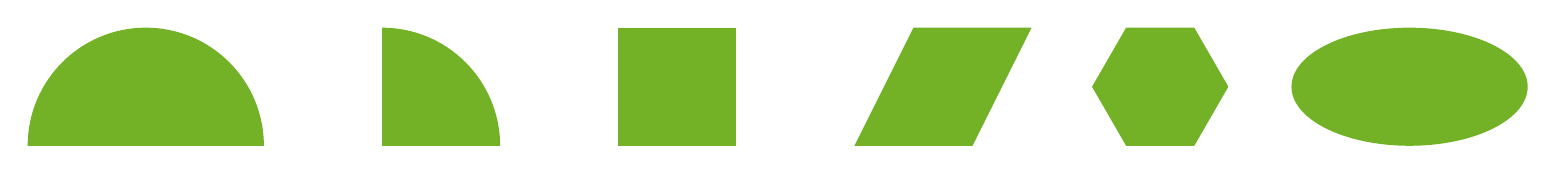
\begin{tikzpicture}[scale=1.5]
        \fill[pasture] (180:1) -- (0:1) arc [start angle=0, end angle=180, radius=1cm];
        \fill[pasture, xshift=2cm] (90:1) -- (0,0) -- (0:1) arc [start angle=0, end angle=90, radius=1cm];
        \fill[pasture, xshift=4cm] (0,0) -- (0,1) -- (1,1) -- (1,0) -- cycle;
        \fill[pasture, xshift=6cm] (0,0) -- (0.5,1) -- (1.5,1) -- (1,0) -- cycle;
        \fill[pasture, xshift=8.3cm, scale=1/sqrt(3)] (0,0) -- ++(0:1) -- ++(60:1) -- ++(120:1) -- ++(180:1) -- ++(240:1) -- cycle;
        \fill[pasture, xshift=10.7cm] (0,.5) ellipse [x radius=1, y radius=.5];
    \end{tikzpicture}
    \problem При помощи трёх собак на привязи <<ограничьте>> козу без привязи так, чтобы выеденный ей участок имел форму равностороннего треугольника.
    \problem При помощи собак <<ограничьте>> непривязанную козу пятиконечной звездой.
    \problem \sub При помощи одной собаки организуйте выпас четырёх коз, привязанных к одному колышку равными по длине верёвками, так, чтобы козам достались равные участки луга. \\
    \sub При помощи пяти собак организуйте выпас четырёх коз без привязи так, чтобы козам достались равные участки луга. \\
    \illustrated{[scale=4]
        \newcommand{\radius}{.4mm}
        \node[peg, label=left:$A$] (A) at (0,0) {};
        \node[peg, label=right:$B$] (B) at (1,0) {};
        \node[peg, label=right:$C$] (C) at (1,1) {};
        \node[peg, label=left:$D$] (D) at (0,1) {};
        \draw (A) -- (B) -- (C) -- (D) -- (A);
        
        \coordinate (G) at (.3,.4);
        \foreach \p/\q in {A/B,B/C,C/D,D/A}{
            \node[ring, opacity=0] (R) at ($(\p)!(G)!(\q)$) {};
            \draw[double, double distance=3pt, line cap=round] (R) -- (G);
            \node[ring] at (R) {};
        };
        \node[goat] at (G) {};
    }{
        \problem \sub Колышки вбиты в вершинах квадрата $ABCD$, между ними натянуты верёвки. Через колечко на ошейнике козы и колечки на верёвках $AB$, $BC$, $CD$, $DA$ продета ещё одна верёвка. В данный момент верёвка натянута. Какова форма участка, на котором коза съест траву?
    } \\
    \sub Та же задача для правильного треугольника. \\
    \sub Та же задача для правильного шестиугольника.
    \problem Колышки вбиты в точках $A$ и $B$, между ними натянута верёвка длины $AB = a$. На верёвку надето колечко $k$. Вторая верёвка длины $b \leq a$ привязана одним концом к колышку $B$, а вторым --- к колечку $k$. Колечко на ошейнике козы $K$ надето на вторую верёвку. На каком участке коза съест траву?
\end{document}